\documentclass[margin=5mm]{standalone}
\usepackage{siunitx}
\usepackage[europeanresistors, RPvoltages]{circuitikz}
%\usepackage[symbols]{circuitikz}
\usepackage{tikz}
\usepackage{xcolor,pgfplots}

\definecolor{volt}{rgb}{0,0,0.7}
\definecolor{curr}{rgb}{0.7,0,0}

\begin{document}

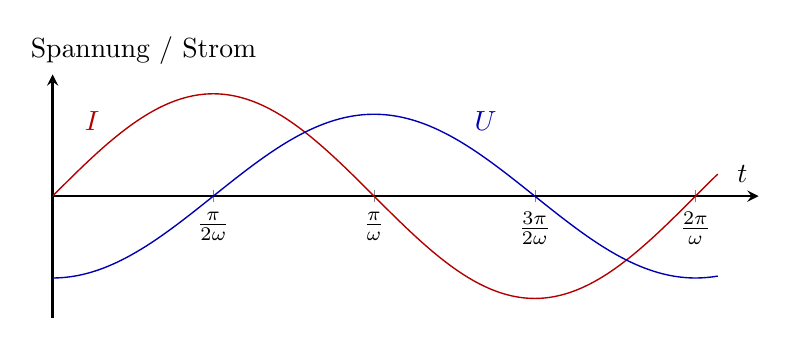
\begin{tikzpicture}
    \begin{axis}[
    axis x line=center,
    axis y line=center,
    xtick={1.5708, 3.1415, 4.7123, 6.283},
    xticklabels={$\frac{\pi}{2\omega}$, $\frac{\pi}{\omega}$, $\frac{3\pi}{2\omega}$, $\frac{2\pi}{\omega}$,},
    %ytick={},
    yticklabels={},
    ytick style={draw=none},
    xlabel={$t_{\vphantom{a}}$},
    ylabel={\hspace*{-.4cm}Spannung / Strom},
    %xlabel style={below right},
    ylabel style={above right},
    xmin=0,
    xmax=6.9,
    ymin=-1.19,
    ymax=1.19,
    axis equal image,
    %scale only axis,
    width = 0.87\linewidth,
    %height = 0.25\linewidth 
    axis line style = thick,
    ]

    Kondensator
    \addplot[domain=0:6.5, samples=500, smooth, curr, line width = .5pt]
    {sin(x*180/3.1415)};
    \addplot[domain=0:6.5, samples=500, smooth, volt, line width = .5pt]
    {0.8*sin(x*180/3.1415-90)};
    \end{axis}
    \draw (0.5,2.5) node{\color{curr}$I$};
    \draw (5.5,2.5) node{\color{volt}$U$};

\end{tikzpicture}


\end{document}
